\documentclass{sig-alternate}
%\documentclass{acm_proc_article-sp}
\usepackage{natbib}
%\usepackage{fancyhdr}
%\pagestyle{fancy}
\setcitestyle{round,aysep={},yysep={;}}

%\usepackage{html}
\usepackage{url}
\usepackage{mymacros}
\usepackage{paralist}
\usepackage{color}
%\usepackage{hyperref}
\graphicspath{{./plot/}}

\hyphenation{c-o-n-t-r-o-l}

\setlength{\textfloatsep}{8pt plus 1.0pt minus 2.0pt}
\setlength{\floatsep}{8pt plus 1.0pt minus 2.0pt}
\setlength{\intextsep}{4pt plus 1.0pt minus 2.0pt}

\begin{document}
\conferenceinfo{WSDM'13,} {February 4--8, 2013, Rome, Italy.} 
\CopyrightYear{2013} 
\crdata{978-1-4503-1869-3/13/02} 
\clubpenalty=10000 
\widowpenalty = 10000
%\fancyhead{}
%\fancyhead[CO,CE]{** To appear in WSDM 2013 **}
\bibliographystyle{plainnat}

\title{Improving the Sensitivity of Online Controlled Experiments by Utilizing Pre-Experiment Data}
\numberofauthors{4} 
\author{
\alignauthor
Alex Deng\thanks{Corresponding authors.}\\
       \affaddr{Microsoft}\\
       \affaddr{One Microsoft Way}\\
       \affaddr{Redmond, WA 98052}\\
       \email{alexdeng@microsoft.com}
\alignauthor
Ya Xu\footnotemark[1]\\
       \affaddr{Microsoft}\\
       \affaddr{1020 Enterprise Way}\\
       \affaddr{Sunnyvale, CA 94089}\\
       \email{yaxu@microsoft.com}
\alignauthor
Ron Kohavi\\
       \affaddr{Microsoft}\\
       \affaddr{One Microsoft Way}\\
       \affaddr{Redmond, WA 98052}\\
       \email{ronnyk@microsoft.com}
\and
\alignauthor
Toby Walker\\
       \affaddr{Microsoft}\\
       \affaddr{One Microsoft Way}\\
       \affaddr{Redmond, WA 98052}\\
       \email{towalker@microsoft.com}
}
\maketitle
\begin{abstract}
Online controlled experiments are at the heart of making data-driven decisions at a diverse set of  companies, including Amazon, eBay, Facebook, Google, Microsoft, Yahoo, and Zynga. Small differences in key metrics, on the order of fractions of a percent, may have very significant business implications.  At Bing it is not uncommon to see experiments that impact annual revenue by millions of dollars, even tens of millions of dollars, either positively or negatively.  With thousands of experiments being run annually, improving the sensitivity of experiments allows for more precise assessment of value, or equivalently running the experiments on smaller populations (supporting more experiments) or  for shorter durations (improving the feedback cycle and agility). We propose an approach (CUPED) that utilizes data from the pre-experiment period to reduce metric variability and hence achieve better sensitivity. This technique is applicable to a wide variety of key business metrics, and it is practical and easy to implement. The results on Bing's experimentation system are very successful:  we can reduce variance by about 50\%, effectively achieving the same statistical power with only half of the users, or half the duration.
\end{abstract}

% A category with the (minimum) three required fields
%Probability and Statistics/Experimental Design: controlled experiments, randomized experiments, A/B testing
\category{G.3}{ Probability and Statistics/Experiment Design}{controlled experiments, randomized experiments, A/B testing}
%A category including the fourth, optional field follows...


\terms{Measurement, Variance, Experimentation}

\keywords{Controlled experiment, Variance, A/B testing, Search quality evaluation, Pre-Experiment, Power, Sensitivity}

\section{Introduction}\label{sec:intro}
%A controlled experiment, also called a randomized experiment, an A/B test, a bucket test or a 1\% experiment, is probably the oldest and the most widely accepted methodology to establish a causal relationship \citep{Mason,Box,Keppel,expsurvey,Manzi}. 

A controlled experiment is probably the oldest and the most widely accepted methodology to establish a causal relationship \citep{Mason,Box,Keppel,expsurvey,Manzi}.  Now widely used and re-discovered by many companies, it is referred to as a randomized experiment, an A/B test \citep{wikipediaABTest}, a split test, a weblab (at Amazon), a live traffic experiment (at Google), a flight (at Microsoft), and a bucket test (at Yahoo!).
%See \citet{causal_book} and \citet{counterfac} for a modern treatment of causal inference and \citet{causal_statsurvay} for recent developments.  
This paper is focused on online controlled experiments, where experiments are conducted on live traffic to support data-driven decisions in online businesses, including e-business sites like Amazon and eBay, portal sites like Yahoo and MSN \citep{expsurvey}, search engines like Microsoft Bing \citep{puzzlingOutcomes} and Google \citep{googlesurvey}. 

Online controlled experiments are critical for businesses. \linebreak Small differences in key metrics, on the order of fractions of a percent, can have very significant business implications.  At Bing it is not uncommon to see experiments that impact annual revenue by millions of dollars, even tens of millions of dollars, either positively or negatively. 
We begin with a motivating example of an online controlled experiment run at MSN \citep{expAtMicrosoft}. MSN Real Estate (\url{http://realestate.msn.com}) had six visual design candidates for the ``Find a home'' widget, as shown in Figure~\ref{fig:msn}. During the experiment, users were randomly split between the 6 variants, where the control is the production version and treatment 1 through 5 are five new designs. The goal was to increase visits to the linked partner sites through the widget. Users' interactions with the widget were instrumented and key metrics such as the number of transfers to partner sites were computed.  In this experiment, the winner, treatment 5, increased revenue from transfer fees by almost $10\%$ compared to the control. 
\begin{figure}[!hbtp]
  \centering
  
\includegraphics[width=.5\textwidth]{msn}
  \caption{Widgets tested for MSN Real Estate.}
  \label{fig:msn}
\end{figure}

One challenge with any controlled experiment is the ability to detect the treatment effect when it indeed exists, usually referred to as ``power'' or ``sensitivity.'' Improving sensitivity is particularly important when running online experiments at large scale. A mature online experimentation platform runs thousands of experiments a year \citep{puzzlingOutcomes,Manzi}. The benefit of any increased sensitivity is therefore amplified by economies of scale. It might seem unnecessary to emphasize sensitivity for online experiments because they tend to have very large sample sizes already (e.g. millions of users \citep{comScore}) and increasing sample size is usually the most straightforward way to improve power. In reality, even with a large amount of traffic, online experiments cannot always reach enough statistical power. Google made it very clear that they are not satisfied with the amount of traffic they have \citep[Slide 6]{googleslide} even with over 10 billion searches per month \citep{comScore}. There are several reasons for this. First, the treatment effects we would like to detect tend to be very small. The sensitivity of controlled experiments is inversely proportional to the number of users squared, so whereas a small site may need 10,000 users to detect a 5\% delta, detecting a 0.5\% delta requires 100 times (10 squared) more users, or one million users. Even a 0.5\% change in revenue per user equates to millions of dollars for large online sites. Second, it is crucial to get results fast. One wants to launch good features early, and more importantly, if the treatment turns out to have a negative impact on users, we need to stop it as soon as possible. Third, there are many experiments that have low triggering rates; that is, only a small fraction of the experiment's users actually experience the treatment feature. For example, in an experiment affecting only recipe-related queries, the majority of the users will not see the target feature because they didn't search for recipes during the experiment. In these cases, the effective sample size can be small and statistical analysis can suffer from low statistical power. 
Finally, in a data-driven culture, there is always demand to run more experiments to keep up with the rate of innovation. A good online experimentation platform should allow many experiments to run together. This also requires that we make optimal use of large but still limited traffic.   


%Statistical hypothesis testing was used to check whether the difference observed among the variants are due to random noise.

%While this particular example illustrates one application of online controlled experiment---testing design changes, online experiment is also widely used in evaluation of back-end changes, such as a performance improvement or an algorithm change.


%Running online experiments effectively and efficiently at large scale is challenging. The problem we address here in particular is regarding statistical sensitivity. To ensure XXX is not due to noise, statstical hypothesis testing
%signal noise ratio, power

 


One way to improve sensitivity is through variance reduction. \citet{expsurvey} provides examples where we can achieve a lower variance using a different evaluation metric or through filtering out users who are not impacted by the change. \citet{choiceofexp} shows how we can use page level randomization at the design stage to reduce variance of page level metrics \citep{Chapelle}. However, these methods are limited in their applicability to special cases and we want a technique that is applicable to any metric as, in practice, businesses are likely to have a set of Key Performance Indicators (KPIs) that cannot be changed easily. Moreover, the technique should preferably not be based on any parametric model because model assumptions tend to be unreliable and a model that works for one metric does not necessarily work for another.

In this paper, we propose a technique, called CUPED \linebreak (Controlled-experiment Using Pre-Experiment Data), which adjusts metrics using pre-experiment data for users in the control and treatment to reduce metric variability.

The key contributions of our work include:
\begin{compactitem}
\item A theoretically sound and practical method to reduce variances for online experiments using pre-experiment data, which greatly increases experiment sensitivity.
\item Extensions of approach to non-user metrics and partially missing pre-experiment data.
\item Criteria for selecting the best covariates, including the empirical result that using the same metric from the pre-experiment typically gives the greatest variance reduction.
\item Validation of the results on real online experiments run at Bing, demonstrating a variance reduction of about 50\%, equivalent to doubling our traffic or halving the time we need to run an experiment to get the same sensitivity.
\item Practical guidance on choices important to successful application of CUPED to real-world online experimentation, including factors like the best length to use for the pre-experiment period and the use of multiple covariates.
\end{compactitem}

\section{Background and Related Work}
\subsection{Analyzing Experiments}
Because of its wide applicability, we focus on the case of the two-sample t-test \citep{studentt,allofstat}. This is the framework most commonly used in online experiment analysis. Suppose we are interested in some metric $Y$ (e.g. Queries per user). To apply the t-test, we assume the observed values of the metric for users in the treatment and control are independent realizations of random variables $Y^{(t)}$ and $Y^{(c)}$. The null hypothesis is that $Y^{(t)}$ and $Y^{(c)}$ have the same mean and the alternative is that they do not. 
The t-test is based on the t-statistic: 
\begin{align}\label{zstat}
\frac{\ybar^{(t)} - \ybar^{(c)}}{\sqrt{\var \left(\ybar^{(t)} - \ybar^{(c)}\right)}},
\end{align}
where $\Delta=\ybar^{(t)} - \ybar^{(c)}$ is an unbiased estimator for the shift of the mean and the t-statistic is a normalized version of that estimator. 
For online experiments, the sample sizes for both control and treatment are at least in thousands, hence the normality assumption on $Y$ is usually unnecessary because of the Central Limit Theorem.

Because the samples are independent, $$\var(\Delta)=\var \left(\ybar^{(t)} - \ybar^{(c)}\right) = \var\left(\ybar^{(t)}\right)+\var\left(\ybar^{(c)}\right).$$ 
In this framework, the key to variance reduction for the difference in mean lies in reducing the variance of the means themselves. As we will see in Section~\ref{sec:varreduction}, this connects our problem to techniques used in Monte Carlo sampling to improve estimation of a mean through variance reduction. 

At a very high level, our proposal for variance reduction works as follows. We conduct the experiment as usual but when analyzing the data, we compute an adjusted or corrected estimate of the delta. That adjusted estimate, $\Delta^*$, incorporates pre-experiment information, such that 
\begin{compactitem}
\item $\Delta^*$ is still an unbiased estimator for the shift in the means (same as $\Delta$), and
\item $\Delta^*$ has a smaller variance than $\Delta$. 
\end{compactitem}
Note that because of the reduced variance, the corresponding t-statistic would be larger for the same expected effect size. We therefore achieved better sensitivity.

\subsection{Linear Models}\label{sec:literature}
We begin with a short review of related work. Variance reduction has been a longstanding challenge for analyzing randomized experiments. The most popular parametric method is based on linear modeling \citep{dagelman}. A linear model for an experiment assumes that the outcome is a linear combination of a treatment effect coupled with additional covariate terms. In particular, suppose $Y_i$ is the outcome metric,  $Z_i$ is the treatment assignment indicator and $\bX_i$ is a vector of covariates. The linear model assumes $\e (Y_i|Z_i,\bX_i) = \theta_0+\delta Z_i + \btheta^T \bX_i$. Under the assumptions of the model, linear regression (also called ANCOVA when covariates are categorical variables) gives a consistent estimator for the average treatment effect and reduces variance. However, the linear model makes strong assumptions that are usually not satisfied in practice, i.e., the conditional expectation of the outcome metric is linear in the treatment assignment and covariates. In addition, it also requires all residuals to have a common variance. 

\subsection{Semi-Parametric Models}
To overcome limitations of the linear model, researchers have developed less restrictive models called semi-parametric models \citep{semipara}, for which Generalized Estimating Equations (GEE) are used for fitting the model. Comparing standard linear models with semi-parametric models, \citet{yangtsiatis} showed that linear model (ANCOVA) and GEE are asymptotically equivalent under the less restrictive semi-parametric model and both give more efficient estimates for the average treatment effect than the unadjusted t-test.  \citet{semiparapretest}, 
\citet{semiparamissing} and \citet{tsiatiscovariateadj} further refined the work using  semi-parametric statistical theory \citep{semipara} and gave the analytical form of a class of estimators for the average treatment effect. This class is complete in the sense that all possible RAL (regular and asymptotically linear) estimators for the average treatment effect are asymptotically equivalent to one in the class. The problem left is to find the estimator in the class with the smallest variance and they provided general guidance. 

In this paper, we look at the problem from a different perspective. By connecting the variance reduction problem in randomized experiments to a similar problem in Monte Carlo simulation, we are able to derive a very powerful result.
Instead of diving into abstract Hilbert spaces and functional influence curves, our argument only involves elementary probability. In particular, we propose to use the data from the pre-experiment period to reduce metric variability, which turns out to be very effective and practically applicable.    


\section{Variance Reduction}\label{sec:varreduction}
Variance reduction is a common topic in Monte Carlo sampling, where the goal is usually to estimate a parameter by repeatedly simulating possible values from the underlying distribution.
%accurately estimate a value by generating many possible values through simulating the underlying distribution. 
In Monte Carlo sampling significant efficiency gains can be had if we use sampling schemes that reduce the variance by incorporating prior information. Unlike Monte Carlo simulations, in the world of online experiments, the population is dynamic and data arrive gradually as the experiment progresses. We cannot design a sampling scheme in advance and then  collect data accordingly. However, we will show that because we have pre-experiment data, we can adapt Monte Carlo variance techniques by applying them ``retrospectively.''

The two Monte Carlo variance reduction techniques we consider here are stratification and control variates. For each technique, we  review the basic concepts and then show how it can be adapted to the online experiment setting.  We devote Section~\ref{sec:combo} to discussing the connections between these two approaches and the implications in practice.

\subsection{Stratification}
Stratification is a common technique used in Monte Carlo sampling to achieve variance reduction. In this section, we show how it can be adapted to achieve the same goal in the world of online experimentation. 


\subsubsection{Stratification in Simulation}\label{sec:stratSim}
The basic idea of stratification is to divide the sampling region into strata, sample within each stratum separately and then combine results from individual strata together to give an overall estimate, which usually has a smaller variance than the  estimate without stratification.

Mathematically, we want to estimate $\e(Y)$, the expected value of $Y$, where $Y$ is the variable of interest. The standard Monte Carlo approach is to first simulate $n$ independent samples $Y_i, i=1,\dots,n,$ and then use the sample average $\ybar$ as the estimator of $\e(Y)$. $\ybar$ is unbiased and $\var(\ybar) = \var(Y)/n$.

Let's consider a more strategic sampling scheme. Assume we can divide the sampling region of $Y$ into $K$ subregions (strata) with $w_k$ the probability that $Y$ falls into the $k$th stratum, $k=1,\dots,K$. If we fix the number of points sampled from the $k$th stratum to be $n_k=n\cdot w_k$, we can define a stratified average to be   
\begin{align}
\yhat_{strat} = \sum_{k=1}^K w_k\ybar_k,\label{eq:stratAve}
\end{align}
where $\ybar_k$ is the average within the $k$th stratum.


The stratified average $\yhat_{strat}$ and the standard average $\ybar$ have the same expected value but the former gives a smaller variance when the means are different across the strata.
%The proof can be found in standard Monte Carlo books (e.g. \cite{stosim}). 
The intuition is that the variance of $\ybar$ can be decomposed into the within-strata variance and the between-strata variance, and the latter is removed through stratification. For example, the variance of children's heights in general is large. However, if we stratify them by their age, we can get a much smaller variance within each age group. 
More formally,
\begin{align*}
\var(\ybar) & =\sum_{k=1}^K\frac{w_k}{n}\sigma^2_k + \sum_{k=1}^K\frac{w_k}{n}(\mu_k - \mu)^2 \\
&\geq \sum_{k=1}^K\frac{w_k}{n}\sigma^2_k =\var(\yhat_{strat})
\end{align*}
where $(\mu_k,\sigma^2_k)$ denote the mean and variance for users in the $k$th stratum. More detailed proof can be found in standard Monte Carlo books (e.g. \cite{stosim}). 
A good stratification is the one that aligns well with the underlying clusters in the data. By explicitly identifying these clusters as strata, we essentially remove the extra variance introduced by them.

%By removing the intrinsic variance not caused by the experiment, we essentially highlight the experiment effect we look for.

\subsubsection{Stratification in Online Experimentation}\label{sec:stratExp}
In the online world, because we collect data as they arrive over time, we are usually unable to sample from strata formed ahead of time. However, we can still utilize pre-experiment variables to construct strata after all the data are collected (for theoretical justification see \citet[Page 153]{stosim}). For example, if $Y_i$ is the number of queries from a user $i$, a covariate $X_i$ could be the browser that the user used before the experiment started. The stratified average in \eqref{eq:stratAve} can then be computed by grouping $Y$ according to the value of $X$,
\begin{align*}
\yhat_{strat} = \sum_{k=1}^K w_k\ybar_k = \sum_{k=1}^K w_k \left(\frac{1}{n_k}\sum_{i:X_i=k}Y_i\right).
\end{align*}
Using superscripts to denote treatment and control groups, 
%the experiment effect is $\delta = \e(Y^{(t)}) - \e(Y^{(c)})$. The two-sample t-test estimates $\delta$ by $\Delta = \ybar^{(t)}- \ybar^{(c)}$ with variance $\var(\ybar^{(t)}) + \var(\ybar^{(c)})$. 
the stratified delta
\begin{align*}
\Delta_{strat} = \yhat_{strat}^{(t)} - \yhat_{strat}^{(c)} = \sum_{k=1}^K w_k(\ybar_k^{(t)}-\ybar_k^{(c)})
\end{align*}
enjoys the same variance reduction as the stratified average in Eq. \eqref{eq:stratAve}.
It is important to note that by using only the pre-experiment information, the stratification variable $X$ is independent of the experiment effect. This ensures that the stratified delta is unbiased.


%For experimentation, it is the difference between the treatment and the control that we care about. 


In practice, we don't always know the appropriate weights $w_k$ to use. In the context of online experimentation, these can usually be computed from users not in the experiment. As we will see in Section~\ref{sec:combo}, when we formulate the same problem in the form of control variates (Section~\ref{sec:cv}), we no longer need to estimate the weights.   

%We have so far demonstrated with one stratification variable $X$. The extension to multiple covariates is straightforward and hence omitted here.

\subsection{Control Variates}\label{sec:cv}
We showed how online experimentation can benefit from the stratification technique widely used in the simulation literature. In this section we show how another variance reduction technique used in simulation, called control variates, can also be adopted in online experimentation. In Section \ref{cvsim}, we review control variates in its original form as a variance reduction technique for simulation. We then show how the same idea can be applied in the context of online experimentation in Section \ref{cvexp}. 

\subsubsection{Control Variates in Simulation}\label{cvsim}
The idea of variance reduction through control variates stems from the following observation. Assume we can simulate another random variable $X$ in addition to $Y$ with known expectation $\e(X)$. In other words, we have independent pairs of $(Y_i, X_i),i=1,\dots,n$. Define 
\begin{align}\label{eq:cv}
\yhat_{cv} = \ybar - \theta\xbar + \theta\e X,
\end{align}
where $\theta$ is any constant. 
$\yhat_{cv}$ is an unbiased estimator of $\e(Y)$ since $- \theta\e(\xbar)+\theta\e(X) = 0$. The variance of $\yhat_{cv}$ is
\begin{align*}
\var (\yhat_{cv}) &= \var (\ybar - \theta \xbar) = \var (Y-\theta X)/n  \\
&=\frac{1}{n} (\var(Y) + \theta^2\var(X) - 2\theta\cov (Y,X)).
\end{align*}
Note that $\var (\yhat_{cv})$ is minimized when we choose 
\begin{align}
\theta = \cov(Y,X)/\var(X)\label{eq:optTheta}
\end{align}
and with this optimal choice of $\theta$, we have 
\begin{align}\label{sim:varred} 
\var (\yhat_{cv}) &= \var(\ybar) (1- \rho^2) ,
\end{align}
where $\rho = \cor (Y,X)$ is the correlation between $Y$ and $X$. Compare  \eqref{sim:varred} to the variance of $\ybar$, the variance is reduced by a factor of $\rho^2$.  The larger $\rho$, the better the variance reduction. The single control variate case can be easily generalized to include multiple variables. 
%The details are included in Appendix~\ref{appendix:multipleCV}. 

It is interesting to point out the connection with linear regression.
The optimal $\btheta$ turns out to be the ordinary least square (OLS) solution of regressing (centered) $Y$ on (centered) $X$,
which gives variance  
\begin{align*} 
\var (\yhat_{cv}) &= \var(\ybar) (1- R^2) ,
\end{align*}
with $R^2$ being the proportion of variance explained coefficient from the linear regression. It is also possible to use nonlinear adjustment. i.e., instead of allowing only linear adjustment as in \eqref{eq:cv}, we can minimize variance in a more general  functional space. Define 
\begin{align}\label{eq:cv2}
\yhat_{cv} = \ybar - \overline{f(X)} + \e(f(X)),
\end{align}
and then try to minimize the variance of \eqref{eq:cv2}. It can be shown that the regression function $\e (Y|X)$ gives the optimal $f(X)$.

\subsubsection{Control Variates in Online Experimentation}\label{cvexp}
Utilizing control variates to reduce variance is a very common technique. The difficulty of applying it boils down to finding a control variate $X$ that is highly correlated with $Y$ and at the same time has known $\e(X)$. 

Although in general it is not easy to find control variate $X$ with known $\e(X^{(t)})$ and $\e(X^{(c)})$, a key observation is that $\e(X^{(t)})-\e(X^{(c)})=0$ in the pre-experiment period because we have not yet introduced any treatment effect. By using only information from before the launch of the experiment to construct the control variate, the randomization between treatment and control ensures that we have $\e X^{(t)}=\e X^{(c)}$.

%All that is required is that $X$ is not affected by the experiment. For example, as we mentioned in Section~\ref{sec:stratExp}, $X$ could be based on information before the launch of the experiment. The randomization between treatment and control ensures that we have $\e X^{(t)}=\e X^{(c)}$.

Given $\e X^{(t)}-\e X^{(c)}=0$, it is easy to see the delta
\begin{align}\label{eq:cvdelta}
\Delta_{cv} &= \yhat_{cv}^{(t)} - \yhat_{cv}^{(c)}
\end{align}
is an unbiased estimator of $\delta=\e(\Delta)$. Notice how $\Delta_{cv}$ does not depend on the unknown $\e (X^{(t)})$ and $\e (X^{(c)})$ at all as they cancel each other. With the optimal choice of $\theta$ from Eq~\eqref{eq:optTheta}, we have that
$\Delta_{cv}$ reduces variance by a factor of $\rho^2$ compared to $\Delta$, i.e.
\begin{align*}
\var(\Delta_{cv}) = \var(\Delta)(1-\rho^2).
\end{align*}
To achieve a large correlation and hence better variance reduction, an obvious approach is to choose $X$ to be the same as $Y$, which naturally leads to using the same variable during pre-experiment observation window as the control variate. As we will see in the empirical results in Section~\ref{sec:emp}, this indeed turns out to be the most effective choice we found for control variates.  

There is a slight subtlety that's worth pointing out. The pair $(Y,X)$ may have different distributions in treatment and control when there is an experiment effect. For $\Delta_{cv}$ to be unbiased, the same $\theta$ has to be used for both control and treatment. The simplest way to estimate it is from the pooled population of control and treatment. The impact on variance reduction will likely be negligible. In the general nonlinear control covariates case, we should use the same functional form in both $\yhat_{cv}^{(t)}$ and $\yhat_{cv}^{(c)}$.

%In fact, as long as the exact same estimate is used in both $\yhat_{cv}^{(t)}$ and $\yhat_{cv}^{(c)}$. 

\subsection{Connection between Stratification and \\Control Variates} \label{sec:combo}
We have discussed two techniques that both utilize covariates to achieve variance reduction. The stratification approach uses the covariates to construct strata while the control variates approach uses them as regression variables.
The former uses discrete (or discretized) covariates, whereas control variates seem more naturally to be continuous variables. It is, however, not surprising that these two approaches are closely related. In fact, we can show that when the covariate $X$ is categorical (say, with discrete values $1,\dots, K$) the two approaches produce identical estimates. Details are included in Appendix~\ref{appendix:combo}. The basic idea is to construct an indicator variable $1_{X=k}$ for each stratum and use it as a control variate with mean  being the stratum weight $w_k$. To this end, the control variates technique is an extension of stratification, where both continuous and discrete covariates are applicable.

While these two techniques are well connected mathematically, they provide different insights into understanding why and how to achieve variance reduction.   
The stratification formulation has a nice analogy with mixture models, where each stratum is one component of the mixture model. Stratification is equivalent to separating samples according to their component memberships, effectively removing the between-component variance and achieving a reduced variance. A better covariate is hence the one that can better classify the samples and align with their underlying structure.
On the other hand, the control variates formulation quantifies the amount of variance reduction as a function of the correlation between the covariates and the variable itself. It is mathematically simpler and more elegant. Clearly, a better covariate should be the one with larger (absolute) correlation. 

%$K$ indicator variables $1_{X=k}$ as control variates with each mean $w_k$. 
%Because we can treat control variates as an extension of stratification, 
%On the other hand, stratification works even if the number of strata is very large, as long as the contribution from individual strata does not dominate the estimate. (add reference XXX). In practice, as many of our metrics are count variables,  
 

\section{CUPED in Practice}\label{sec:practice}
%We have now established  the basic framework for CUPED.
%using pre-experiment data to reduce variance. 

 
A simple yet effective way to implement CUPED is to use the same variable from the pre-experiment period as the covariate. 
Indeed, this is essentially what we have implemented in practice for Bing's experimentation system.  However, there are situations when this is not possible or practical. 
For example,  if we want to measure user retention rate or conduct an experiment on new users, there are no pre-experiment data to work with. In fact, in most online experiments, we may not have pre-experiment information on \textit{all} users. An additional challenge is how to use pre-experiment data for metrics whose analysis unit is not a user. This section is devoted to address practical challenges like these using Bing's experimentation system as a case study. 
%At the end of this section, we also discuss how to handle metrics with analysis units that are not ``user.''
%In this section, we turn to some of the practical challenges we may face in real online experiments using Bing's experimentation system as a case study.

\subsection{Selecting Covariates}
The choice of covariates is critical, as it directly determines the effectiveness of variance reduction. With the choice of the right variables we can halve the variance but with the wrong choice there is little reduction in variance. To understand which pre-experiment variables worked best we evaluated a large number of possible pre-experiment variables. Across a large class of metrics, our results consistently showed that using the same variable from the pre-experiment period as the covariate tends to give the best variance reduction. In addition, the lengths of the pre-experiment and the experiment periods also play a role. Given the same pre-experiment period, extending the length of the experiment does not necessarily improve the variance reduction rate. On the other hand, a longer pre-period tends to give a higher reduction for the same experiment period. We discuss more details in the context of an empirical example in Section~\ref{sec:emp}.   

\subsection{Handling Missing Pre-Experiment Data}
In online sites, we might not have pre-experiment data on all users in the experiment. This can occur because some users are visiting for the first time, or users simply do not visit the site frequently enough to appear during the pre-experiment period. In addition, users are identified by cookies, which are unreliable and can ``churn'' (i.e. change due to users clearing their cookies).

This poses a challenge for using the pre-experiment information to construct covariates. For users who are in the experiment but not in the pre-experiment period, the corresponding covariates are not well-defined. One way to address this is to define another covariate that indicates whether or not a user appeared in the pre-experiment period. With this additional binary covariate, we can set the missing covariate values to be any constant we like. Intuitively, this is equivalent to first splitting users into two strata: those that appeared in the pre-experiment period and those that did not. Note that for the stratum of users with pre-experiment data, their pre-experiment covariates are well-defined so further variance reduction based on these covariates is possible. In addition, the stratification by presence in the pre-period is a further source of variance reduction. 

\subsection{Beyond Pre-Experiment Data}\label{sec:beyond}
So far we only considered reducing metrics variability based on covariates constructed using the pre-experiment data. This is not only because using the same variable from the pre-period tends to give the best variance reduction, but also because the pre-experiment information is guaranteed to be independent of the experiment's effect, which is crucial to avoid biased results.   

It is probably easier to demonstrate this mathematically with the control variates formulation. In Eq.~\eqref{eq:cvdelta}, the delta $\Delta_{cv}$ is computed assuming $\e(X^{(t)})=\e(X^{(c)})$. If there is truly a difference between control and treatment in terms of $X$ and this equality does not hold, $\Delta_{cv}$ will be biased. For example, we know a faster page load-time usually leads to more clicks on a search page \citep{expsurvey}. If we use the number of clicks as the covariate in an experiment that improves page load-time, we will end up underestimating the experiment impact on the load-time because part of the improvement is ``adjusted away'' by the covariate. See Section \ref{sec:emp} for a real example of biased results caused by using a covariate that violates the requirements described here. 

However, this does not mean that covariates based on pre-experiment data are the only choice. 
All that is  required is that the covariate $X$ is not affected by the experiment's treatment. A natural extension is the class of covariates constructed using information gathered at the first time a user appears in the experiment. For instance, the day-of-week a user is first observed in the experiment is independent of the experiment itself. Such covariates can serve as an additional powerful source for variance reduction. To further extend this idea, covariates based on any information established before a user actually \textit{triggers} the experiment feature are also valid. This can be particularly helpful if the feature to be evaluated has a low triggering rate.

%or a user's demographic information are both

\subsection{Handling Non-User Metrics}\label{sec:nonUser}
As we mentioned in Section~\ref{sec:intro}, in online experiments, users (cookies) are the common randomization unit. In the discussion thus far, we have assumed that the analysis unit is also ``user.'' However, this is not always the case. For example, we may want to compute click-through-rate (CTR) as the total number of clicks divided by the total number of pages. The analysis unit here is  a ``page'' instead of a ``user.''  Variance estimation itself is harder when there is a mismatch between the analysis unit and the experiment unit. The most common solution is to use the delta method to produce correct estimate of variance that takes into account the correlation of pages from the same user \citep{choiceofexp,googlesurvey,expsurvey}. To achieve variance reduction for these non-user level metrics, we need to combine the delta method and our variance reduction techniques together. The details are provided in Appendix~\ref{appendix:deltamethod}. In fact, not only can the metric of interest (e.g. CTR) be at page level, we can have page-level covariates as well. This opens the door to a larger class of covariates that are based on features specific to a page that may be not specific to a user, e.g. time stamp on a page-view.

\section{Empirical Results}\label{sec:emp}
In this section, we share empirical results that show the effectiveness of CUPED for Microsoft Bing's experimentation system. 
%In the rest of this section, we share several studies to show the effectiveness of CUPED in practice at Bing. 
First we show how CUPED can greatly improve the sensitivity for a real experiment run at Bing. Next we look deeper into a 3-week A/A test, which is a controlled experiment where treatment is identical to control and hence the treatment effect is known to be $0$. Using an A/A experiment we can examine important decisions that can have a large impact of the success of variance reduction for real-world online experimentation. Finally, we show how biased estimates  arise if we go past the user triggering into the experiment and choose a covariate inappropriately. 
\\
\\
\subsection{Slowdown Experiment in Bing}
\begin{figure}[!b]
  \centering
  \includegraphics[width=.5\textwidth]{pfdelayPCRhalftime.eps}
  \includegraphics[width=.5\textwidth]{pfdelayPCRhalfuser.eps}
  \caption{Slowdown experiment. Top: p-value. Bottom: p-value when using only half the users for CUPED.}
  \label{fig:pfdelay}
\end{figure}
To show the impact of CUPED in a real experiment we examine an experiment that tested the relationship between page load-time and user engagement on Bing. Delays, on the order of hundreds of milliseconds, are known to hurt user engagement \citep[Section 6.1.2]{expsurvey}.  In this experiment, we deliberately delayed the server response to Bing queries by 250 milliseconds. The experiment first ran for two weeks on a small fraction of Bing users, and we observed an impact to click-through-rate (CTR) that was borderline statistically significant, i.e., the p-value was just slightly below our threshold of 0.05.  To confirm that the treatment effect on this metric is real and not a false positive, a much larger experiment was run, which showed that this was indeed a real effect with a p-value of 2e-13. 
% This example represents a common scenario. 
%economizing on use of limited traffic for an experiment results in borderline significant p-values.   

We applied CUPED using CTR from the 2-week pre-period as the covariate. The result is impressive: the delta was statistically significant from day 1!  The top plot of Figure \ref{fig:pfdelay} shows the p-values over time in log scale. The black horizontal line is the 0.05 significance bar. The vanilla t-test trends slowly down and by the time the experiment was stopped in 2 weeks, it barely reached the threshold. When CUPED is applied, the entire p-value curve is below the bar. The bottom plot of Figure \ref{fig:pfdelay} compares the p-value curves when CUPED runs on only half the users. 
Even with half the users exposed to the experiment, CUPED results in a more sensitive test, allowing for more non-overlapping experiments to be run.   While most experiments are not known to be negative to the user experience a-priori, it has been well documented that most experiments are flat or negative \citep{expAtMicrosoft, Manzi}, so being able to run experiments with the same statistical power on smaller populations of users is very important.

%It is clear that even when only half the users are available for CUPED, the benefit from variance reduction makes up for the sample size loss. In other words, this real example shows that indeed we can save half of our traffic with CUPED. 
Applying CUPED to other experiments at Bing has resulted in similar increases to statistical power.

%/
%The first experiment is to test the effect of slower page loading time to user engagement. It is widely accepted that several milliseconds of delay could hurt user engagement. In this experiment, we deliberately slow down users' page loading time(PLT) by 250ms. The experiment ran for 2 weeks on a small fraction of Bing traffic and we observed a boundary significant impact on Page-Click-Rate(PCR), i.e, p-value only slightly below $0.05$. We then collected 2 weeks pre-experiment period data and use that as the covariate. With the help of variance reduction, we got statistically significant results from day 1! Top plot of Figure \ref{fig:pfdelay} shows the evolution of t-statistics for both cases as we ran the experiment longer and longer. When t-statistics is above $1.96$ or below $-1.96$, we claim that a nonzero treatment effect exists with 95\% confidence. Hence $\pm 1.96$ are the significance thresholds. In this experiment, the variance reduced t-statistics curve is below the significance threshold for the whole period. On the other hand, without variance reduction, the t-statistics shows a slow downward trend but still linger around $-1.96$. In other words, with variance reduction, we could stop the experiment in just a few day if our sole purpose is to verify the PCR impact. Similarly, we can reduce the sample size and yet still achieve the same sensitivity. Bottom plot of Figure \ref{fig:pfdelay} shows the t-statistics curve when we pretend we only have half of the sample size. In this case variance reduced t-statistics actually still show slightly larger absolute t-statistics. This real example shows that indeed we can save half of our traffic with this technique. 
%/


%
%The first experiment is a test on a known treatment effect and we have stat-significant results even without using variance reduction. In the next example variance reduction actually changed our decision from non-stat-significant result to a stat-significant one. In this experiment, feature team want to test a new ranking algorithm and want to see whether the new algorithm could make user query more. The metric of interest here is Queries per user(Queries/UU). Top plot in Figure \ref{fig:QueriesPerUUTrueAB} shows the t-statistics over experiment length. Before applying variance reduction, the t-statistics curve is always below the significance line. We then applied control variates with 1 week pre-experiment data as covariate. This time the t-statistics curve climbed above the significance line after the 15th day. A similar plot(omitted here) shows with $60\%$ of sample size, variance reduced t-statistics already performs at par with the normal t-statistics using all samples. 
%
%\begin{figure}[!hbtp]
%  \centering
%  \includegraphics[width=.5\textwidth]{queriesPerUUtstatTRUEABsixtyUser}
%  \caption{Ranking experiment: p-value}
%  \label{fig:QueriesPerUUTrueAB}
%\end{figure}

\subsection{Factors Affecting CUPED Effectiveness}
In this section we look at factors that can have a large impact on the success of using CUPED in practice. The data we use here are from a 3-week A/A experiment. 
%\begin{compactenum}[1)]
%\item the covariates, using pre-experiment metric of interest alone or combine it with other covariates;
%\item the length of the experiment;
%\item the length of the pre-experiment if pre-experiment data is used as covariates;
%\item user level metrics and page level metrics.
%\end{compactenum}

\subsubsection{Covariates}
Figure \ref{fig:QueriesPerUU} shows CUPED's variance reduction rate for the metric queries-per-user. Two covariates are considered: (1) entry-day, which is a categorical variable indicating the first day a user appears in the experiment and (2) queries-per-user in the 1-week pre-experiment period. Note that the entry-day is not pre-experiment data, but it satisfies the condition required in Section \ref{sec:beyond} because the treatment has no effect on when a user will come for the first time during the experiment. 
%A generalized definition of pre-experiment period for any user could be the time period before the user is recruited in the experiment, e.g. the first entry event. Under this generalized definition, entry-day can be viewed as pre-experiment data. 
\begin{figure}[!hbtp]
  \centering
  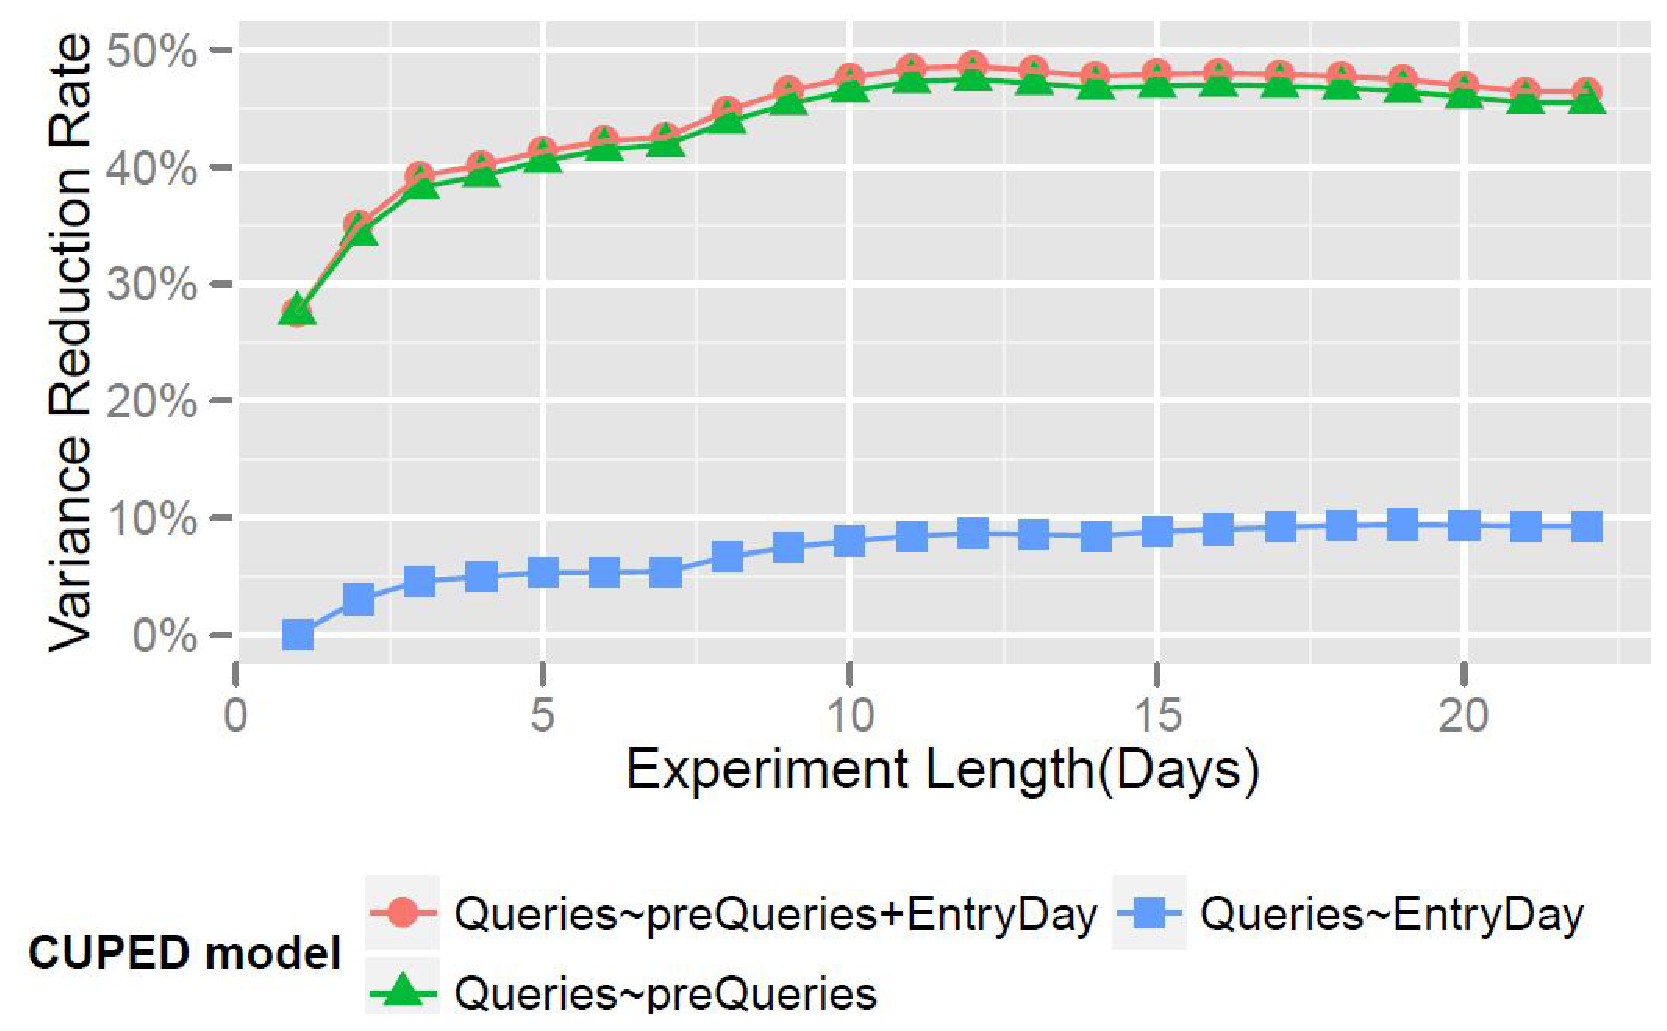
\includegraphics[width=.5\textwidth]{queriesPerUUVarRed.eps}
  \caption{Variance reduction for Queries/UU using different covariates.}
  \label{fig:QueriesPerUU}
\end{figure}

Note that the full experiment ran for 3 weeks, but the reduction rate is evaluated and plotted as the experiment accumulates data up until to the full 3 weeks. From the plot we can see that when only entry-day is used as the covariate, the variance reduction rate increases as the experiment runs longer and stays at about 9\% to 10\% after 2 weeks. On the other hand, using only the pre-experiment period queries-per-user, variance reduction rate can reach more than 45\%.  When we combine the two covariates together, we only gain an extra 2\% to 3\% more reduction compared to the pre-experiment queries-per-user alone. This suggests that the same metric computed in the pre-experiment period is a better single covariate. That is intuitive since the same metric in the experiment and pre-experiment periods should naturally have high correlation. The fact that when combining two covariates together the marginal variance reduction is small means most correlation between entry-day and queries-per-user can be ``explained away'' by the pre-experiment queries-per-user. More precisely, the partial correlation between entry-day and queries-per-user given pre-experiment queries-per-user is low.

\subsubsection{Lengths of Experiment and Pre-Experiment}\label{sec:twoconflicting}
In addition to the effect of covariates, Figure~\ref{fig:QueriesPerUU} also provides insights on the impact of the experiment length.
An interesting observation is that the variance reduction rate for the pre-experiment covariate (green/triangle) is not monotonically increasing as the experiment duration increases. It reaches the maximum at about 2 weeks and then starts to slowly decrease. To help understand the underlying reasons for this trend, we plot 4 variations of this curve with pre-period length varying from 3 days to 2 weeks. As shown in Figure~\ref{fig:QueriesPerUUperiod}, we see that a longer pre-period gives a higher variance reduction rate. 
\begin{figure}[!hbtp]
  \centering
 \includegraphics[width=.5\textwidth]{queriesPerUUVarRedPeriod.eps}
  \caption{Impact of pre-experiment period length.}
  \label{fig:QueriesPerUUperiod}
\end{figure}

The trends in Figure \ref{fig:QueriesPerUU} and \ref{fig:QueriesPerUUperiod} together reveal two conflicting factors that impact the effectiveness of CUPED.
\begin{compactitem}
\item \emph{Correlation}. The higher the correlation, the better the variance reduction. When we increase the pre-experiment period length or increase the experiment duration, the correlation increases for ``cumulative'' metrics such as queries-per-user. This is because the longer the period, the higher the signal-to-noise ratio.
\item \emph{Coverage}. Coverage is the percentage of users in the experiment that also appeared in the pre-experiment period. Coverage is determined by:
\begin{compactitem}
\item \emph{Experiment Duration}. As the experiment duration increases, coverage decreases. The reason is that frequent visitors are seen early in the experiment and users seen later in the experiment are often new or ``churned'' users. The result is that as coverage decreases, the rate of variance reduction goes down. 
\item \emph{Pre-period Duration}. Increasing the pre-period length increases coverage because we have a better chance of matching an experiment user in the pre-period.
\end{compactitem}
\end{compactitem}
When pre-experiment period was chosen to be 2 weeks, the variance reduction rate is about $50\%$ for a large range of experiment durations. 

\subsubsection{Metric of Interest}
Besides the choice of covariates and the lengths of experiment and pre-experiment, CUPED effectiveness varies from metric to metric, depending on the correlation between the metric and its pre-experiment counterpart. We applied \linebreak CUPED on a few metrics, such as clicks-per-user and visits-per-user. CUPED performed well on all these metrics with similar variance reduction curves as in Figure \ref{fig:QueriesPerUU}. One notable exception is revenue-per-user, where CUPED reduced the variance by less than 5\% due to the low correlation of revenue-per-user between the pre-experiment and the experiment periods. We also applied CUPED on a few page level metrics (see the discussion in Section~\ref{sec:nonUser}). Figure \ref{fig:pcr} shows the reduction rate for click-through-rate (CTR), using 2-week pre-experiment CTR as the CUPED covariate. Figure \ref{fig:correlation} plots the correlation curve between the two periods. Both the variance reduction rate and the correlation are similar to those of queries-per-user. 
\begin{figure}[!hbtp]
  \centering
  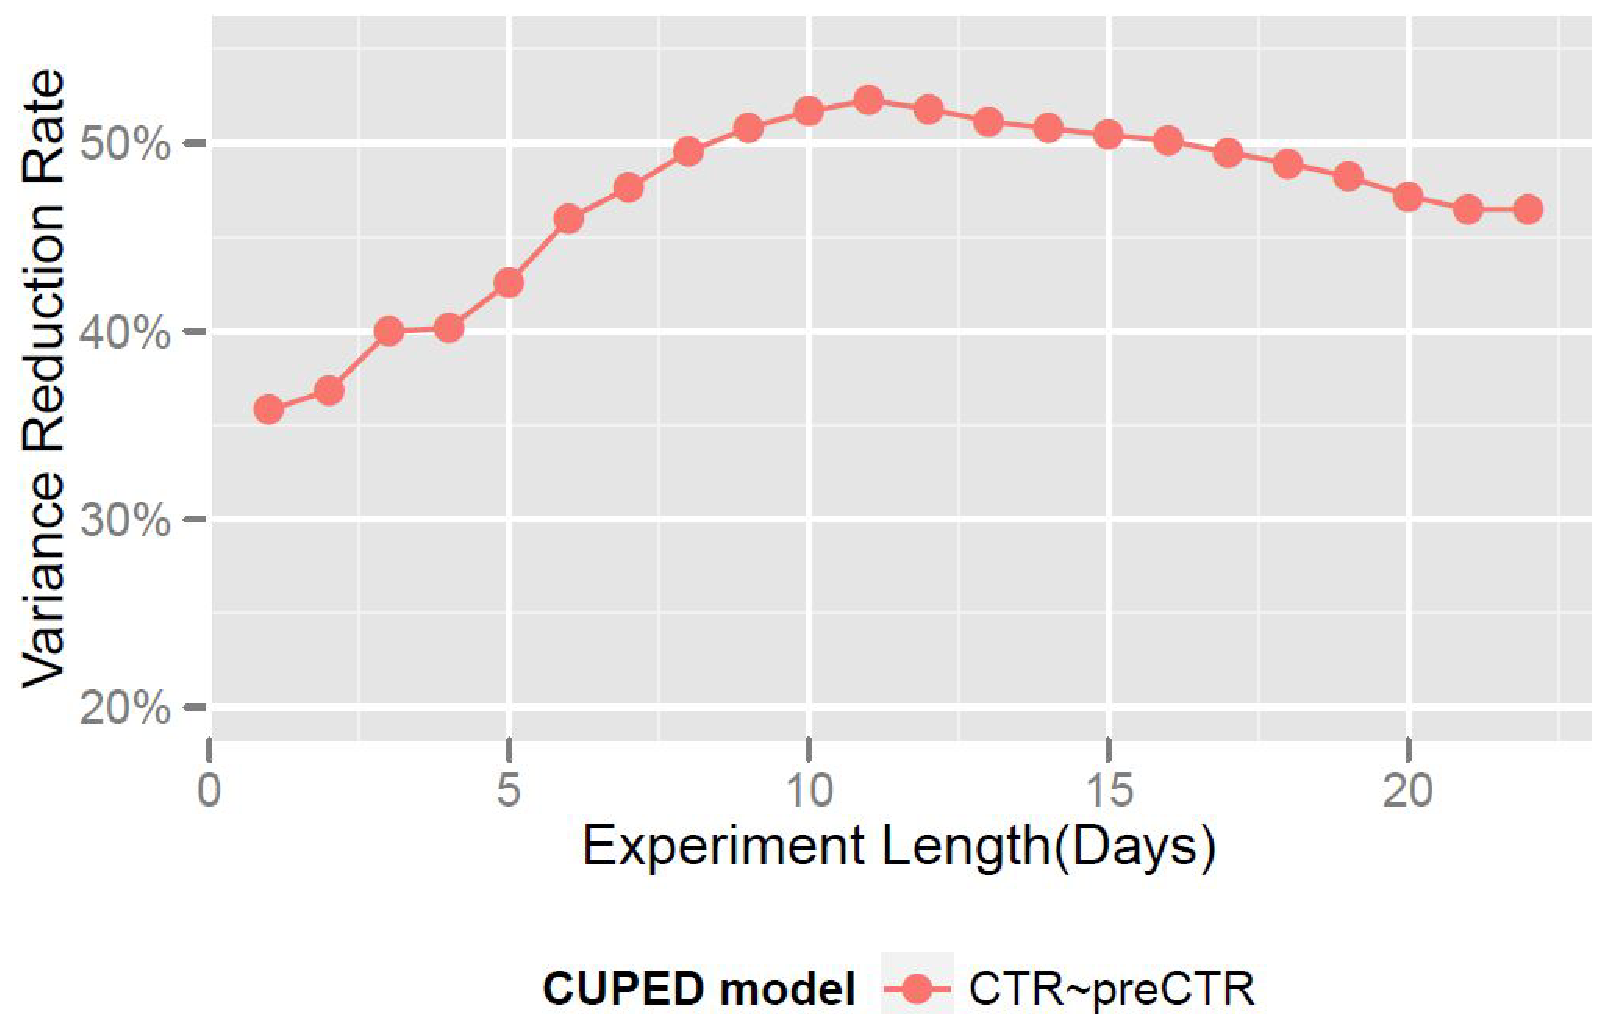
\includegraphics[width=.5\textwidth]{pcr.eps}
  \caption{Variance reduction rate for CTR.}
  \label{fig:pcr}
\end{figure}
\begin{figure}[!hbtp]
  \centering
  \includegraphics[width=.5\textwidth]{correlation.eps}
  \caption{Correlation between the metrics of interest and their covariates within the matched users.}
  \label{fig:correlation}
\end{figure}


%We have so far studied the effectiveness of CUPED on the metric queries-per-user. 
%It is not surprising that the metric of interest itself can have a big impact on the effectiveness as well.
%We look into the two properties of queries-per-user that may explain the effectiveness:
%%Queries-per-user has the following two properties that may explain effective variance reduction: 
%(1) Queries-per-user has high inertia over time. A heavy user last week is likely to continue to be heavy this week; 
%%(2) It is ``cumulative,'' because the number of queries from a user increases (or cumulates) over a longer time period; 
%(2) Queries-per-user is defined at user level. 
%Other similar metrics include sessions-per-user, clicks-per-user, etc.
%
%\textit{Inertia.} Inertia affects variance reduction since it directly determines the correlation between the metric and its pre-experiment counterpart. In our applications, we found \linebreak CUPED did not work well on some metrics due to lack of inertia. Revenue-per-user, for example, only showed less than 5\% variance reduction. Intuitively, this is because revenue depends highly on whether a user's search intention is monetizable. If a user searched for a well monetizable query such as ``car insurance'' last week, it is unlikely that the same user will search for ``car insurance'' again this week.
%
%%\textit{Cumulativeness.} The ``cumulative'' characteristic affects CUPED effectiveness by impacting the contribution of the two conflicting factors introduced in \ref{sec:twoconflicting}. For ``cumulative''  metrics such as queries-per-user, the increasing correlation usually dominates the two for the first few weeks. As a result CUPED performs well on these metrics with decent variance reduction rates. Things are quite different for bounded metric such as percentage of users who signed in. Even though the metric has high inertia, the value on user level is binary and as coverage drops, new users contributes more and more to the variance because the contribution from matched user does not grow. In this case, we found the variance reduction rate quickly drops as coverage drops.
%
%\begin{figure}[!hbtp]
%  \centering
%  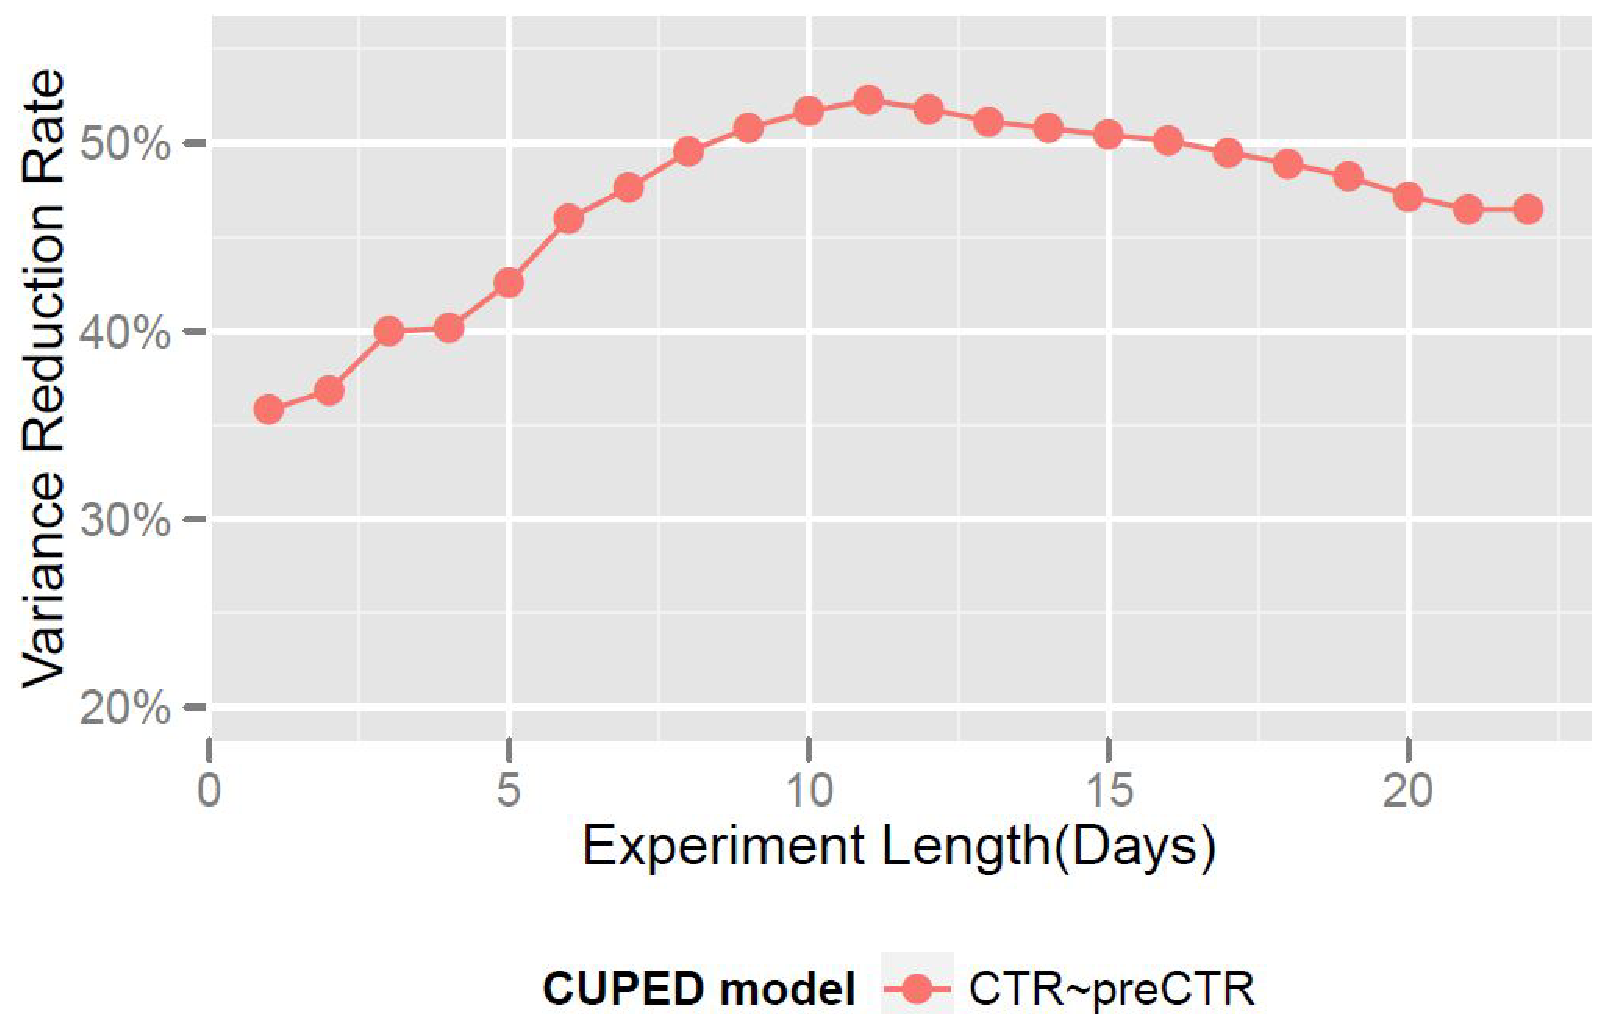
\includegraphics[width=.5\textwidth]{pcr.eps}
%  \caption{Variance reduction rate for CTR.}
%  \label{fig:pcr}
%\end{figure}
%\begin{figure}[!hbtp]
%  \centering
%  \includegraphics[width=.5\textwidth]{correlation.eps}
%  \caption{Correlation between the metrics of interest and their covariates within the matched users.}
%  \label{fig:correlation}
%\end{figure}
%
%\textit{User level vs. page level.}  Because CUPED relies on user level correlation to achieve variance reduction, one may expect it to be more effective for user level metrics such as queries-per-user and clicks-per-user than for page level metrics such as click-through-rate (CTR). Figure \ref{fig:pcr} shows the reduction rate for CTR, using 2-week pre-experiment CTR as the CUPED covariate. It is surprising at first to see a similar reduction rate as that of queries-per-user. To explain the similarity, we plot the correlation between CTR and the pre-experiment CTR among the \textit{matched users} in Figure~\ref{fig:correlation}. Notice how the CTR correlation is similar to the correlation for queries-per-user. The reason that page level metrics such as CTR can have such high correlation is because CTR can be reformulated as the sum of clicks \textit{per user} divided by the sum of page-views \textit{per user}. This user level representation is exactly why a page level metric can enjoy a high variance reduction rate as well.  
%, the numerator is ``cumulative''. In other words, CUPED's effectiveness on a page level metric relies on whether the numerator is ``cumulative'' in its user level representation. 

%The distinction of user level and non-user level is also important for the variance and covariance calculation (see \citet{choiceofexp}, \citet{googlesurvey} and Appendix~\ref{appendix:deltamethod}).
 
\subsection{Warning on Using Post-Triggering Data}
In Section \ref{sec:practice}, we mentioned that to guarantee unbiased results, any covariate $X$ has to satisfy the condition $\e(X^{(t)})=\e(X^{(c)})$. We illustrate this point in Figure \ref{fig:QueriesPerUUWrong}. The data is from another Bing experiment, where queries-per-user increased statistically significantly. If we were to look for a metric with high correlation to queries-per-user, there is actually a much better candidate than the pre-experiment queries-per-user: the ``in-experiment'' Distinct Queries-per-user (DQ-per-user).  DQ is defined as query counts for a user after consecutive duplicated queries are removed. As a result, DQ is extremely highly correlated with queries-per-user. Seemingly, DQ-per-user as covariate sounds like a good idea. However, Figure \ref{fig:QueriesPerUUWrong} shows that the CUPED estimates $\Delta_{CUPED}$ are negative and the confidence intervals are almost always below $0$ (Note how narrow the confidence intervals are. DQ-per-user indeed reduced variance a lot!). This suggests the queries-per-user difference between the treatment and control is negative with 95\% confidence, a result that is directionally opposite of the known effect. The contradiction is only apparent because DQ-per-user does not satisfy $\e(X^{(t)})=\e(X^{(c)})$. In fact, since we know treatment has larger queries-per-user, it has larger DQ-per-user too. By \eqref{eq:cvdelta}, CUPED estimate $\Delta_{cv}$ can be interpreted as the in-experiment delta for the metric of interest ``corrected'' by the delta for the covariate. In this case the covariate delta is also positive, driving down the CUPED estimate below $0$. This example illustrates the pitfall when extending CUPED beyond using pre-experiment (or pre-triggering) data. 
\begin{figure}[!hbtp]
  \centering
  \includegraphics[width=.5\textwidth]{queriesPerUUDeltaWrongAB.eps}
  \caption{Example where results are directionally incorrect when covariates violate the pre-triggering requirement.}
  \label{fig:QueriesPerUUWrong}
\end{figure}


\section{Conclusions}\label{sec:conclusion}

%Increasing the sensitivity of online experiments allows for more precise assessment of value, or equivalently running the experiments on smaller populations (supporting more non-overlapping experiments) or for shorter durations (improving the feedback cycle and agility).  We introduced CUPED, a new technique for increasing the sensitivity of controlled experiments by utilizing pre-experiment data.  Actual experiments on Bing showed that variance can be reduced by about 50\%, effectively achieving the same statistical power with only half the users, or half the duration.

Increasing the sensitivity of online experiments allows for more precise assessment of value, or equivalently running the experiments on smaller populations (supporting more non-overlapping experiments) or for shorter durations (improving the feedback cycle and agility). We introduced CUPED, a new technique for increasing the sensitivity of controlled experiments by utilizing pre-experiment data. CUPED is currently live in Bing's online experimentation system. Three important recent experiments showed variance reductions of  45\%, 52\% and 49\% with one week of experiment and one week of pre-experiment data. This reassures that CUPED can indeed help us effectively achieve the same statistical power with about only half the users, or half the duration.

CUPED is widely applicable to organizations running online experimentation systems because of its simplicity, ability to be added easily to existing systems, and its support for metrics commonly used in online businesses. Based on our experience applying CUPED at Bing, we can make the following recommendations for others interested in applying CUPED to their online experiments: 
\begin{compactitem}
\item Variance reduction works best for metrics where the distribution varies significantly across the user population. One common class of such metrics where the value is very different for light and heavy users. Queries-per-user is a paradigmatic example of such a metric.
\item Using the metric measured in the pre-period as the covariate typically provides the best variance reduction.
\item Using a pre-experiment period of 1-2 weeks works well for variance reduction. Too short a period will lead to poor matching, whereas too long a period will reduce correlation with the outcome metric during the experiment period. 
\item Never use covariates that could be affected by the treatment, as this could bias the results.  We have shown an example where directionally opposite conclusions could results if this requirement is violated.
\end{compactitem}
While CUPED significantly improves the sensitivity of online experiments, we would like to explore improvements: 
\begin{compactitem}
\item \emph{Optimized Covariate Selection}. Extend CUPED to optimize the selection of covariates, both for particular metrics and for particular types of experiments (e.g., a backend experiment might use data center as a covariate). We also plan to study the theory and practice to optimize selection of multiple covariates from a large library of potential covariate variables. 
\item \emph{Incorporating Covariate Information into Assignment}. Rather than adjusting the data after the experiment completes, if we can make randomization aware of covariates we can potentially improve  the sensitivity of our experiments even more as well as allocating traffic more efficiently to experiments. 
\end{compactitem}



%In the world of online experimentation making experiments as sensitive as possible is critical to drive rapid -- detecting successes and failures as fast as possible -- and ensuring we can accurate measure even small changes on key KPIs is critical. CUPED, a new technique for variance reduction using pre-experiment, supports both goals by greatly increase the sensitivity of our experiments. Our results show that CUPED can effectively halve the sample size required to achieve the same sensitivity as a standard experiment analysis.
%
%We believe the ideas behind CUPED are widely applicable to organizations running online experiments. For example, CUPED applies to the most common analysis technique for online experiments -- two-sample t-tests. Furthermore, CUPED is easily added to existing experiment systems as it only requires the use of aggregate data commonly generated by such systems. 
%
%To apply CUPED in practice we extended the basic technique to deal with key challenges including missing data, non-user metric and go beyond strictly pre-experiment covariates to include a more generalized set of ``pre-experiment'' variables. 
%
%Based on our experience we can make the following recommendations for applying CUPED to online experiments: 
%
%\begin{itemize}
%\item Variance variation works best for metrics whose variances is high across the user population. One common class of such metrics where the value is very different for low intensity and high intensity users. queries-per-user is a paradigmatic example of such a metric.
%\item Using the metric measured in the pre-period as the covariate typically provides the best variance reduction.
%\item Never use covariates that are affected by the treatment. While this may seem obvious there are more insidious examples waiting for the unwary experimenter.  
%\item Using a pre-experiment period of 1-2 weeks works well for variance reduction. Too short a period will lead to poor matching whereas too long a period will reduce correlation with the outcome metric during the experiment period. 
%\end{itemize}
%
%While CUPED significantly improves the sensitivity of online experiments, we would like to explore several avenues in future work:
%
%\begin{itemize}
%\item Automatic Covariate Selection. In future work we hope to automatically select the covariates used for each metric's covariate adjustment.  
%\item Incorporating Covariate Information into Assignment. Rather than adjusting the data after the experiment completes, if we can make randomization aware of covariates we can potentially improve  the sensitivity of our experiments even more. Doing this dynamically, at scale, is challenging and represents an exciting area of future work. 
%\end{itemize}

\section{Acknowledgments}
We wish to thank Sam Burkman, Leon Bottou, Thomas Crook, Kaustav Das, Brian Frasca, Xin Fu, Mario Garzia, Li-wei He, Greg Linden, Roger Longbotham, Carlos Gomez Uribe, Zijian Zheng and many members of the Bing Data Mining team.
%
% The following two commands are all you need in the
% initial runs of your .tex file to
% produce the bibliography for the citations in your paper.

\bibliography{sigproc}  % sigproc.bib is the name of the Bibliography in this case
% You must have a proper ".bib" file
%  and remember to run:
% latex bibtex latex latex
% to resolve all references
%
% ACM needs 'a single self-contained file'!
%
%APPENDICES are optional
%\balancecolumns
%\pagebreak
\newpage
\appendix
%Appendix A

\section{Control Variates as an extension of Stratification}\label{appendix:combo}
Here we show that when the covariates are categorical, stratification and control variates produce identical results.

For clarity and simplicity, we assume $X$ is binary with values 1 and 0. Let $w=\e(X)$. The two estimates are
\begin{align*}
\yhat_{strat}&=w\ybar_1 + (1-w)\ybar_0,\\
\yhat_{cv} &= \ybar -\hat{\theta}\xbar +\hat\theta w,
\end{align*}
where $\ybar_1$ denotes the average of $Y$ in the $\{X=1\}$ stratum and $\hat\theta=\wh{\cov}(Y,X)/\wh{\var}(X)=\ybar_1 -\ybar_0$. 
Plugging in the expression for $\hat\theta$, we have
\begin{align*}
\yhat_{cv} &= \ybar -(\ybar_1 -\ybar_0)\xbar +(\ybar_1 -\ybar_0)w\\
&= (1-\xbar)\ybar_0 + \ybar_0\xbar +(\ybar_1 -\ybar_0)w\\
& = w\ybar_1 + (1-w)\ybar_0 = \yhat_{strat},
\end{align*}
where the second equality follows from the fact that $\ybar=\xbar\ybar_1 + (1-\xbar)\ybar_0$. 

To prove for the case with $K>2$, we construct $K-1$ indicator variables as control variates. 
With the observation that the coefficients $\hat\theta_k=\ybar_k-\ybar_0$, the proof follows the same steps as the binary case outlined above.   

\section{Generalization to Other Analysis Unit}\label{appendix:deltamethod}
As we mentioned in Section~\ref{sec:practice}, to achieve variance reduction for non-user level metrics, we need to incorporate delta method. The formulation we lay out in Section~\ref{sec:varreduction} makes it easy to achieve this, as we will see below. 
  
We use CTR as an example and derive for the control variates formulation since it's more general. 

Let $n$ be the number of users (non-random). Denote $Y_{i,j}$ the number of clicks on user $i$'s $j$th page-view during the experiment and $X_{i,k}$ the number of clicks on user $i$'s $k$th page-view during the pre-experiment period.  
Let $N_{i}$ and $M_{i}$ be the numbers of page-views from user $i$ during the experiment and pre-experiment respectively. The estimate for CTR in Eq.~\eqref{eq:cv} using $X_{i,j}$ as the control variate  becomes
\begin{align*}
\yhat_{cv}&=\frac{\sum_{i,j}Y_{i,j}}{\sum_{i,j}1}-\theta\frac{\sum_{i,k}X_{i,k}}{\sum_{i,k}1}+\theta\e(X_{i,k})\\
&=\frac{\sum_{i}Y_{i,+}}{\sum_{i}N_i}-\theta\frac{\sum_{i}X_{i,+}}{\sum_{i}M_i}+\theta\e(X_{i,j}),
\end{align*}
where $Y_{i,+}=\sum_jY_{i,j}$ is the total number of clicks from user $i$. Similar notation applies to $X_{i,+}$.

Following the same derivation as in Section~\ref{cvsim}, we know $\var(\yhat_{cv})$ is minimized at
\begin{align}
\theta&=\cov\left(\frac{\sum_{i}Y_{i,+}}{\sum_{i}N_i},\frac{\sum_{i}X_{i,+}}{\sum_{i}M_i}\right)/\var\left(\frac{\sum_{i}X_{i,+}}{\sum_{i}M_i}\right)\nonumber\\
&\doteq\cov\left(\frac{\ybar}{\mu_N}-\frac{\mu_Y\overline{N}}{\mu_N^2}-\frac{\mu_Y}{\mu_N}, \frac{\xbar}{\mu_M}-\frac{\mu_X\overline{M}}{\mu_M^2}-\frac{\mu_X}{\mu_M}\right)\nonumber\\
 &\qquad /\var\left(\frac{\xbar}{\mu_M}-\frac{\mu_X\overline{M}}{\mu_M^2}-\frac{\mu_X}{\mu_M}\right)\nonumber\\
& = \cov\left(\frac{\ybar}{\mu_N}-\frac{\mu_Y\overline{N}}{\mu_N^2}, \frac{\xbar}{\mu_M}-\frac{\mu_X\overline{M}}{\mu_M^2}\right)/\var\left(\frac{\xbar}{\mu_M}-\frac{\mu_X\overline{M}}{\mu_M^2}\right)\label{eq:thetaDelta}
\end{align} 
where the second equality follows from using Taylor expansion to linearize the ratios and $\ybar=\frac{1}{n}\sum_{i}Y_{i,+}$ with $\mu_Y=\e(\ybar)$ (similarly for $\mu_X$, $\mu_N$ and $\mu_M$). 

Because the user is the randomization unit and user level observations are i.i.d., we have 
\begin{align*}
\sqrt{n}\left(\ybar, \overline{N},\xbar, \overline{M}\right)\Rightarrow N(\mu, \Sigma),
\end{align*} 
following a multivariate normal distribution with mean vector $\mu$ and covariance matrix $\Sigma$ easily estimated from the i.i.d. samples. 

It is now straight forward to estimate $\theta$ in Eq.~\ref{eq:thetaDelta} using
\begin{align*}
\theta = (\beta_1^T\Sigma\beta_2)/(\beta_2^T\Sigma\beta_2),
\end{align*}
where $\beta_1=(1/\mu_N, -\mu_Y/\mu_N^2, 0, 0)^T$ and \\$\beta_2=(0,0,1/\mu_M, -\mu_X/\mu_M^2)^T$ are the coefficients in Eq.~\ref{eq:thetaDelta}. 

Note that in the example above, both the metric of interest (CTR) and the covariate metric are at page-view level. We can easily see that the derivation works generally for various combinations. The metric can be at user level while the covariate can be at page-view level, etc. This opens door to a whole new class of covariates which are based on features specific to a page not to a user. Finally, it is easy to see that the case with multiple control variates follow similarly. 
\end{document}


%%%%%%%%%%%%%%%% this is notes area %%%%%%%%%%%%%%%%%%%%%%%%%%%%%%
\section{stratified average}\label{appendix:stratMeanVar}
We now show that the stratified average has the same expected value as the standard average but with a smaller variance.
\begin{align}
\e(\yhat_{strat}) &=\sum_{k=1}^K w_k\e\left(\ybar_k\right)=\sum_{k=1}^K w_k\mu_k=\mu \equiv \e(\ybar)\nonumber\\
\var(\yhat_{strat}) &= \sum_{k=1}^Kw_k^2\var(\ybar_k)= \sum_{k=1}^K\frac{w_k^2}{n_k}\sigma^2_k \label{stratVar}
\end{align}
where $(\mu_k,\sigma^2_k)$ denote the mean and variance for users in the $k$th segment. On the other hand,
\begin{align}
\var(\ybar) = \frac{1}{n}\sigma^2 = \sum_{k=1}^K\frac{w_k}{n}\sigma^2_k + \sum_{k=1}^K\frac{w_k}{n}(\mu_k - \mu)^2 \geq \sum_{k=1}^K\frac{w_k}{n}\sigma^2_k \label{var}
\end{align}
where the second equality follows by decomposing the total variance $\sigma^2$ into within-segment variance and between-segment variance.
If users in each segment are sampled strictly according to the probabilities $w_k$, we have $w_k=n_k/n$ ignoring the round-off errors. Combining \eqref{stratVar} and  \eqref{var}, we get
\begin{align*}
\var(\ybar) \geq \var(\ybar_{strat}). 
\end{align*} 

\section{Multiple Control Variates}\label{appendix:multipleCV}
We show here how to generalize from the single covariate to multiple covariates in the control variates formulation.
 
Let $\bX = (X_1,X_2, \dots, X_m)^T $ be a random vector of $m$ random variables
% and suppose we simulated $n$ independent samples from $(Y, X_1,X_2, \dots, X_m)$, denoted by $(Y_j, X_{1,j},X_{2,j}, \dots, X_{m,j}),j=1,\dots,n$.
Define
\[
\yhat_{cv} = \ybar - \theta^T\bxbar +\theta^T\e \bX,
\]
where $\theta$ is a $m\times 1$ vector of constants, $\bxbar = (\xbar_1,\xbar_2,\dots,\xbar_m)^T$ and $\e \bX = (\e X_1, \e X_2,\dots,\e X_m)^T$. The optimal constant vector $\theta$ is the ordinary least square (OLS) solution of the regression problem 
\[
Y = \theta_0 + \theta^T \bX.
\]
The closed-form solution of $\theta$ is well-known in any book covering OLS \citep{allofstat}. Also, 
\begin{align}\label{sim:varred2} 
\var (\yhat_{cv}) &= \frac{1}{n} \var Y (1- R^2) ,
\end{align}
where $R^2$ is the $R^2$ coefficient of the regression fit, which stands for proportion of variance explained by the regression model(\citet{allofstat}).
In particular, when $m=1$, this reduces to univariate regression problem and the solution is  $\theta =  \cov(Y,X)/\var(X)$, $R^2 = \rho^2$ .


Denote $Y_i$ the variable we want to measure on user $i$ and let $X_i$ be a covariate, with $i=1,\dots,n$. For example, $Y_i$ could be the number of queries from user $i$ during the experiment period and $X_i$ could be the browser the user used at the time he/she enters the experiment. 

Let's consider the case where $X_i\in\{1,\dots,K\}$ is discrete and can take $K$ possible values. Based on the values of $X_i$'s, we can group all users into $K$ segments. Let $w_k=\p(X_i=k)$ be the probability that a user falls into the $k$th segment. We can define a stratified average to be
\begin{align*}
\ybar_{strat} = \sum_{k=1}^K w_k\ybar_k = \sum_{k=1}^K w_k \left(\frac{1}{n_k}\sum_{i:X_i=k}Y_i\right),
\end{align*}
where $n_k$ denotes the number of users in the $k$th segment.



 Define
\begin{align}
\yhat^{(g)}_{cv} &=  \ybar^{(g)} - \theta\xbar^{(g)}, \quad g = c,t  \ , \label{yhatexp}\\
\Delta_{cv} &= \yhat_{cv}^{(t)} - \yhat_{cv}^{(c)}.
\end{align}

Given $\e X^{(t)}-\e X^{(c)}=0$, it is easy to see $\Delta_{cv}$ is unbiased estimator of $\delta$:
\begin{align*}
\e \Delta_{cv} &= \e \ybar^{(t)} - \e \ybar^{(c)} - \theta (\e\xbar^{(t)} - \xbar^{(c)} )\\
& = \delta - (\e X^{(t)} - \e X^{(c)}) = \delta . 
\end{align*}
Moreover, with appropriate $\theta$, $\Delta_{cv}$ benefit from variance reduction comparing to $\Delta$ since
\begin{align*}
\var \Delta_{cv} & = \var \yhat^{(t)}_{cv}+\var \yhat^{(c)}_{cv}\\
& < \var \ybar^{(t)}+\var \ybar^{(c)} = \var \Delta\ .
\end{align*}

To get the optimal $\theta$, under null hypothesis, $(Y^{(t)}, X^{(t)})$ and  $(Y^{(c)}, X^{(c)})$ follows the same distribution law. We have shown in Section \ref{cvsim} that the optimal $\theta$ is $\cov (Y,X)/\var X$ where superscript is omitted since it does not matter.  With the optimal $\theta$ and follows the same argument as in  Section \ref{cvsim}, 
\begin{align*}
\var\Delta_{cv} = \var \Delta \times (1-\rho^2),
\end{align*}
where $\rho$ is the correlation between $Y$ and $X$.

Extension to multiple control variates is also straightforward. \eqref{yhatexp} is changed to 
\begin{align}\label{yhatmulti}
\yhat^{(g)}_{cv} =  \ybar^{(g)} - \theta^T\bxbar^{(g)}, \quad g = c,t\ ,
\end{align}
and $\theta$ is the least square solution of the regression $Y = \theta_0 + \theta^T \bX$ for control (or treatment under the null hypothesis). 



